\chapter{Conclusões, Trabalhos Futuros e Cronograma}\label{cap:conclusao} 

Este capítulo abordará as conclusões dessa  proposta de mestrado referentes aos resultados do capítulo \ref{cap:resultados},  bem como uma seção de Trabalhos Futuros e  Cronograma. Na seção de Conclusão serão feitas considerações finais dos resultados de cada base de dados apresentadas, e logo após, em Trabalhos Futuros tem a pretenção de melhorar e expandir tudo que fora realizado  nesta pesquisa, e expor que existe uma continuidade para todo esse estudo aqui elaborado. Já no Cronograma, será criado uma tabela temporal onde esta será divida em meses e tarefas definindo os passos a serem seguidos até a conclusão da dissertação.

\section{Conclusão}\label{cond}
No capítulo \ref{cap:resultados} foram aplicados algoritmos supervisionados em algumas bases de dados a fim de provar se o problema  de rotulação de dados visto por este  trabalho foi solucionado. Uma vez conhecido o problema, foi executado dois algoritmos supervisionados servindo de amostra para provar que era possível fazer rotulação de dados com estes algoritmos (Naive Bayes e CART), tema deste trabalho. E já comparando ao trabalho de rotulação de clusters elaborado por \citeonline{LOPES2014} utilizando o algoritmo de Redes Neurais, este estudo demonstra de forma empírica a execução de outros algoritmos com paradigmas diferentes, para provar que essa técnica também funciona com outros algoritmos supervisionados testados.

Como o cerne da pesquisa é a rotulação de dados, foram apresentados dois algoritmos com paradigmas diferentes, e em ambos, suas execuções nas bases de dados resultaram em respostas satisfatórias no âmbito da rotulação. Embora os rótulos encontrados  em cada base de dados não tenham sido totalmente idênticos, tanto um algoritmo como outro mostraram semelhanças em vários rótulos gerados, como exemplo das bases IRIS e GLASS.

O processo de rotulação é composto por um, ou vários atributos, de maior relevância entre eles junto com sua(s) faixa(s) de valor(es) que mais se repetem, contéudo já visto na subseção \ref{cap:ferramentas:ssec:rotulacao}. Seguindo esse modelo foram adicionadas a cada resultado tabelas mostrando em porcentagem o grau de correlacionamento entre os atributos. Essas tabelas tem como objetivo de passar o comportamento dos atributos através da aplicação da técnica de  correlação entre eles na escolha do atributo rótulo.

No modelo de resolução proposto foi inicialmente utilizado na base de dados Seeds o algoritmo Naive Bayes (seção \ref{cap:resultados:ssec:seed:nb}). Onde inicialmente foi escolhido um ou vários atributos que tiveram maior valor no resultado da aplicação da técnica de correlação dos atributos na tabela  \ref{tab:execucoes:seed:nb}. Após a escolha do atributo que fará parte do rótulo, o segundo passo é a escolha da faixa de valores do atributo. Essa segunda etapa é dependente totalmente da discretização, visto na seção \ref{cap:refTeor:sec:discret}, e independente da primeira etapa. O método é capaz de gerar a faixa de maior repetição de valores de qualquer atributo, mas nesta pesquisa  a faixa escolhida é do atributo rótulo. Para ter mais  confiabilidade  no rótulo o método escolhe a faixa de valores que mais se repetem. No caso desse algoritmo o resultado na tabela \ref{tab:rot:seeds:nb} consegue provar uma boa eficiência, pois em cada 70 elementos do cluster 1, somente 14, ficaram de fora dessa faixa. No cluster 2, somando os dois atributos rótulos tem-se 12 elementos que não estão dentro da representatividade do rótulo. Outro valor pequeno em relação aos 70 elementos. E no cluster 3, somente 5 elementos não estão dentro da faixa considerada rótulo.


\begin{figure}[h!]
    \centering
    \subfloat[Naive Bayes]{
        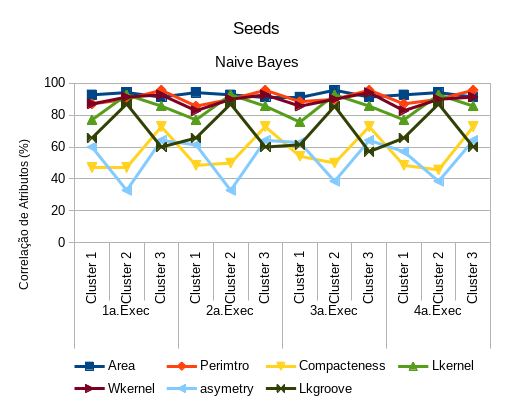
\includegraphics[scale=.8]{figs/grafico_NB_SEED_exec_grp.png}
        \label{fig:execucoes:nb} }
    \quad
    \subfloat[CART]{
        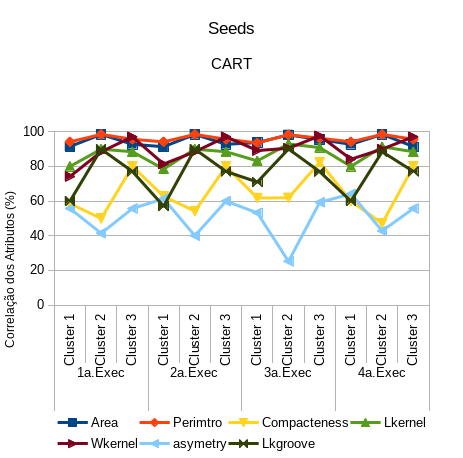
\includegraphics[scale=.8]{figs/grafico_CART_SEED_exec_grp.png}
        \label{fig:execucoes:cart} }
    
    \caption{Gráfico de Execuções dos algoritmos supervisionados na base de dados SEEDS.} \label{fig:graf:SEED_NB_CART}
        
        %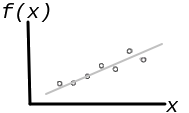
\includegraphics[scale=0.4]{figs/grafB.png}
        %\caption{Polinômio Superajustado} \label{grafB}
\end{figure}


No cenário da execução do algoritmo CART, os resultados foram diferentes dos  apresentados pelo Naive Bayes, mas nem por isso foram insatisfatórios. Contudo uma breve análise sobre as execuções das tabelas ~\ref{tab:execucoes:seed:nb} e \ref{tab:execucoes:seed:cart} podem ser observadas nos gráficos da figura  \ref{fig:graf:SEED_NB_CART}. O comportamento dos valores do correlacionamento dos atributos ao longo das execuções mostram-se equilibradas, figura \ref{fig:execucoes:cart}. O gráfico do CART tem um movimento semelhante ao do aplicado do Naive Bayes (figura \ref{fig:execucoes:nb}), embora a variável \textbf{asymetry} saia um pouco do padrão nada alterou nos rótulos, pois seus valores são baixos, contudo  o valor de \textbf{perimetro} ficou bastante encostado ao valor da \textbf{area}, fazendo o rótulo \textbf{perimetro} aparecer nos grupos 1 e 2. E também só não foi escolhido pelo grupo 3 , pois  a variável \textbf{Wkernel} estava com valor mais alto. E no gráfico percebe-se que  \textbf{Wkernel} mantém valores altos em todas as execuções do grupo 3.

De acordo com o exposto no parágrafo anterior pode-se dizer sobre os resultados que o Naive Bayes acabou sendo um pouco melhor, pois no que diz respeito ao número de elementos fora da faixa definida pelo rótulo, o CART acabou por ter mais elementos fora da faixa de rótulo comparado aos resultados do Naive Bayes. Isso implica dizer que o rótulo deixa de representar mais elementos usando o CART ao invés do Naive Bayes, em outras palavras, o Naive Bayes representou mais elementos concordante com o rótulo do que o CART.


\begin{figure}[h!]
    \centering
    \subfloat[Naive Bayes]{
        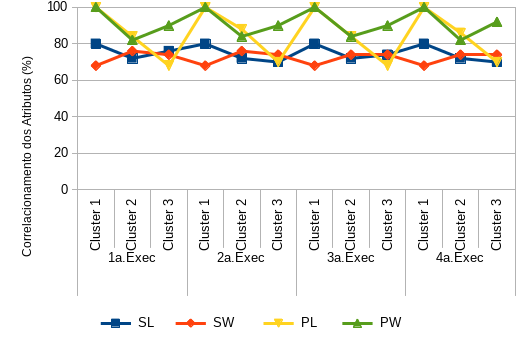
\includegraphics[scale=.9]{figs/grafico_NB_IRIS_exec_grp.png}
        \label{fig:graf:IRIS_NB} }
    \quad
    \subfloat[CART]{
        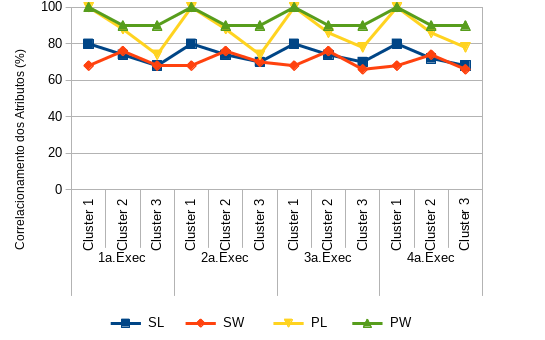
\includegraphics[scale=.9]{figs/grafico_CART_IRIS_exec_grp.png}
        \label{fig:graf:IRIS_CART} }
    
    \caption{Gráfico de Execuções dos algoritmos supervisionados na base de dados IRIS.} \label{fig:graf:IRIS_NB_CART}
        
        %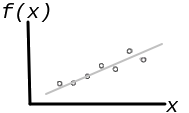
\includegraphics[scale=0.4]{figs/grafB.png}
        %\caption{Polinômio Superajustado} \label{grafB}
\end{figure}

Já na base de dados IRIS, os dois algoritmos supervisionados testados apresentaram os mesmos rótulos nos clusters 1 e 3. Nos gráficos da figura \ref{fig:graf:IRIS_NB_CART} pode-se acompanhar como os valores dos atributos se comportam em seus clusters nas quatro execuções. 

Os algoritmos aplicados na base IRIS tem resultados nos gráficos bastantes semelhantes ao da base SEEDS, e logo percebe-se que a base IRIS contêm características que possuem mais atributos bem correlacionados em relação ao da base SEEDS, pois nenhum atributo possui valor abaixo da linha 65(\%) de relacionamento entre eles. Embora no gráfico as  linhas referentes aos comportamentos dos atributos  nos clusters 1 e 3 não sejam totalmentes iguais em cada figura (\ref{fig:graf:IRIS_NB} e \ref{fig:graf:IRIS_CART}), não  modificou o resultado dos rótulos como resposta.

Conforme resultados das tabelas \ref{tab:rot:iris:nb} e \ref{tab:rot:iris:cart} aprensentadas pela execução dos dois algoritmos os rótulos escolhidos no cluster 1 foram dois atributos: \textbf{petalwidth} e  \textbf{petallength}. Onde cada um deles definiram faixas de valor que foi possível abranger 100\% dos elementos. Já no cluster 2 cada algoritmo teve um atributo rótulo diferente, e embora não tivesse a mesma acurácia do cluster 1, obteve um total, de 86\% de acurácia e deixando de representar 7 elementos do rótulo \textbf{petallength} pelo Naive Bayes, e 84\% de acurácia deixando de representar 8 elementos do rótulo \textbf{petalwidth} com CART. E no cluster 3 o atributo escolhido para compor o rótulo foi o \textbf{petalwidth} em ambos os algoritmos. Logo percebe-se a importância do atributo rótulo no cluster 3,  pois o rótulo representa 45 elementos no total de 50 dentro do cluster, deixando somente 5 elementos fora dessa faixa representada pelo rótulo.

%A repetição do atributo \textbf{petalwidth} em todos os rótulos, acaba mostrando o grau de relevância desse atributo na base de dados. Para um especialista é interessante saber que esse atributo possue um grande referencial na base de dados. Nos rótulos esse atributo assumiu faixas diferentes conseguindo assim o método da um significado ao cluster. 


\begin{figure}[!h]
    \centering
    \subfloat[Execução 1]{
        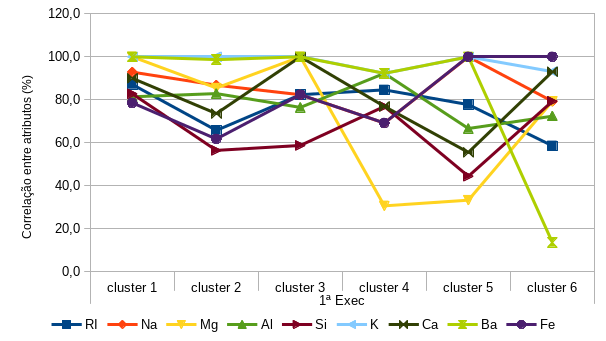
\includegraphics[scale=.4]{figs/grafico_NB_Glass_exec_grp_1.png}
        \label{fig:graf:GLASS_NB_1} }
    \hspace{0.5cm}
    \subfloat[Execução 2]{
        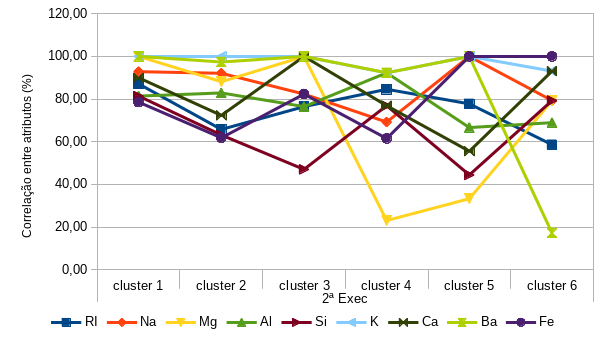
\includegraphics[scale=.4]{figs/grafico_NB_Glass_exec_grp_2.png}
        \label{fig:graf:GLASS_NB_2} }
    \hspace{0.5cm}
    \subfloat[Execução 3]{
        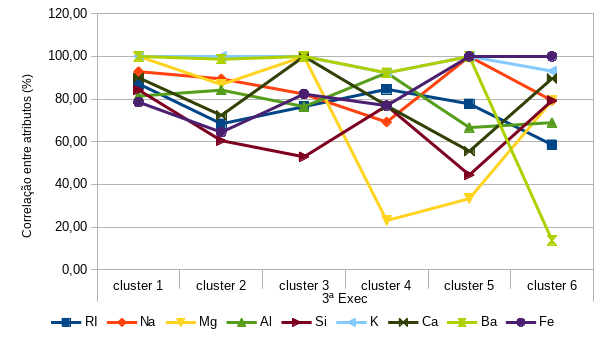
\includegraphics[scale=.4]{figs/grafico_NB_Glass_exec_grp_3.png}
        \label{fig:graf:GLASS_NB_3} }
    \hspace{0.5cm}
    \subfloat[Execução 4]{
        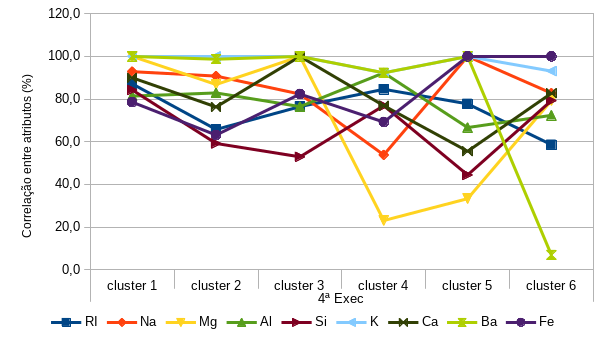
\includegraphics[scale=.4]{figs/grafico_NB_Glass_exec_grp_4.png}
        \label{fig:graf:GLASS_NB_3} }
    \caption{Gráfico de Execuções do algoritmo supervisionado Naive Bayes na base de dados GLASS.} \label{fig:graf:NB}
        
        %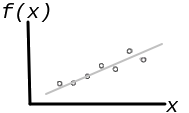
\includegraphics[scale=0.4]{figs/grafB.png}
        %\caption{Polinômio Superajustado} \label{grafB}
\end{figure}

\begin{figure}[!h]
    \centering
    \subfloat[Execução 1]{
        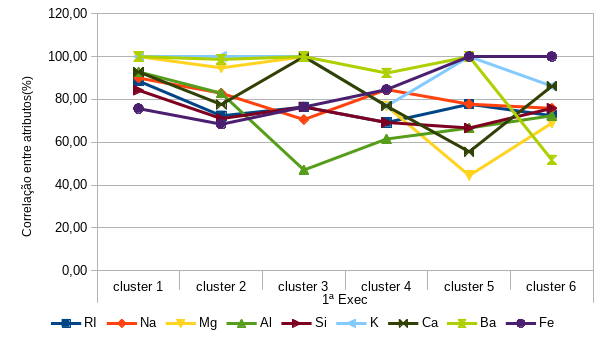
\includegraphics[scale=.4]{figs/grafico_CART_GLASS_exec_grp_1.png}
        \label{fig:graf:GLASS_CART_1} }
    \hspace{0.5cm}
    \subfloat[Execução 2]{
        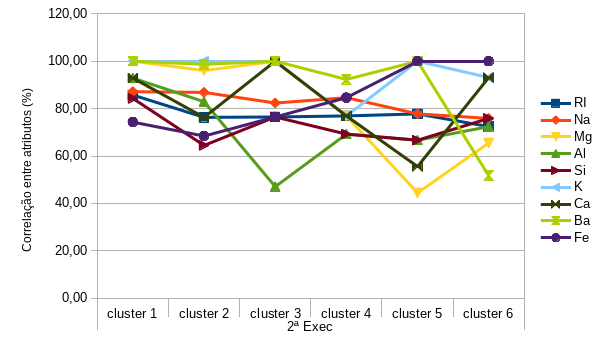
\includegraphics[scale=.4]{figs/grafico_CART_GLASS_exec_grp_2.png}
        \label{fig:graf:GLASS_CART_2} }
    \hspace{0.5cm}
    \subfloat[Execução 3]{
        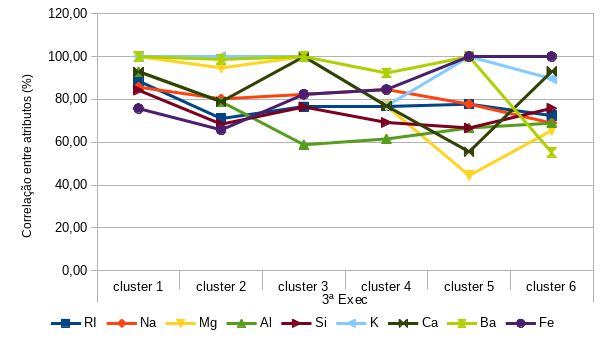
\includegraphics[scale=.4]{figs/grafico_CART_GLASS_exec_grp_3.png}
        \label{fig:graf:GLASS_CART_3} }
    \hspace{0.5cm}
    \subfloat[Execução 4]{
        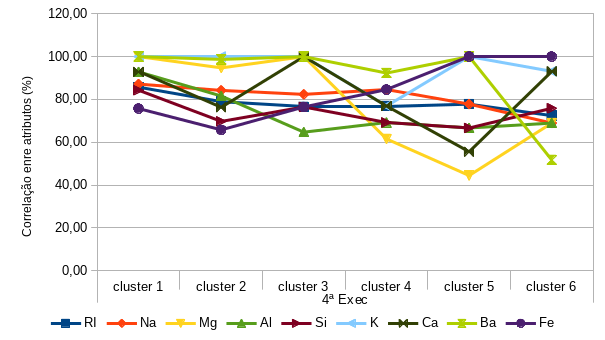
\includegraphics[scale=.4]{figs/grafico_CART_GLASS_exec_grp_4.png}
        \label{fig:graf:GLASS_CART_4} }
    
    \caption{Gráfico de Execuções do algoritmo supervisionado CART na base de dados GLASS.} \label{fig:graf:CART}
        
        %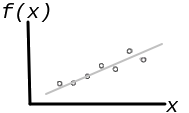
\includegraphics[scale=0.4]{figs/grafB.png}
        %\caption{Polinômio Superajustado} \label{grafB}
\end{figure}

A avaliação da base de dados GLASS referente a rotulação apresentada na tabela \ref{tab:rot:glass:nb} do Naive Bayes, não foi tão bem sucedida quanto ao CART. Dos seis clusters definidos na rotulação somente dois deles não tiveram 100\% de acurácia, e dentre esses dois clusters foi onde obtiveram os mais baixos valores de acurácia.

%No cluster 4 em comparação aos dois algoritmos testados, houve uma diferença no Naive Bayes por apresentar três atributos compondo o rótulo, como pode ser visto na tabela \ref{tab:execucoes:glass:nb}, diferente do algoritmo CART que apresentou somente um atributo - \textbf{Ba} - também presente no rótulo do Naive Bayes. Se o rótulo for composto por três atributos o registro tem que apresentar os atributos que façam parte das faixas rótulos para poderem serem representados pelo rótulo. No CART por apresentar somente um atributo e sua faixa, acaba  mitigando o erro, pois só é necessário que cada registro seja compatível com somente uma faixa do rótulo, para ser representado, uma maior porcentagem de acurácia.

Nos gráficos da figura  \ref{fig:graf:NB} e \ref{fig:graf:CART} são aprensentados os comportamentos de correlacionamento dos atributos rótulos do Naive Bayes e CART respectivamente, e mesmo havendo semelhança nos gráficos os valores de correlação dos atributos no CART foram melhores, e por conseguinte teve melhor acurácia comprovado no gráfico \ref{fig:graf:grafico_NB_CART_acuracia}.

Como conclusão, foi constatado nesta pesquisa que quanto melhores são balanceados os clusters, melhores são os resultados com o algoritmo estatístico Naive Bayes. Podendo ser comprovado nas bases SEEDS e IRIS. Já  na base GLASS que é uma base mais desbalanceada  pode-se notar que na figura \ref{fig:graf:CART}, de execuções do CART, há um comportamento dos clusters melhor que no Naive Bayes. Então através de testes foi detectado que o método de rotulação de dados quando em bases mais balanceadas tiveram melhores resultados com algoritmo estatístico, e quando em bases não tão balanceadas, obtiveram melhores resultados com o algoritmo de árvore de decisão. Isso pode ser constatado no gráfico \ref{fig:graf:grafico_NB_CART_acuracia}, onde o Naive Bayes só perde nos clusters da base GLASS.

Por fim, ao analisar os resultados após a aplicação dos dois algoritmos supervisionados pode-se afirmar que é possível fazer rotulação de cluster, conforme resultados demonstrado na figura \ref{fig:graf:grafico_NB_CART_acuracia}. Através desta figura visualiza-se uma acurácia de 80\% na maioria dos resultados, provando que os rótulos encontrados representam bem os clusters testados. %E uma obsevação técnica dos algoritmos utilizados é que o CART se mostrou bem mais rápido em relação ao Naive Bayes para gerar os resultados.

\begin{figure}[h!]
    \centering
  %  \subfloat[Naive Bayes]{
  %      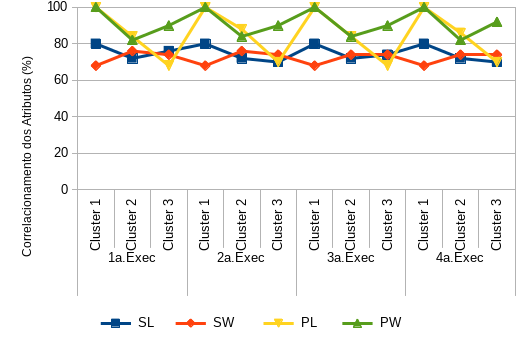
\includegraphics[scale=0.8]{figs/grafico_NB_IRIS_exec_grp.png}
  %      \label{fig:graf:IRIS_NB} }
  %  \quad
  %  \subfloat[CART]{
  %      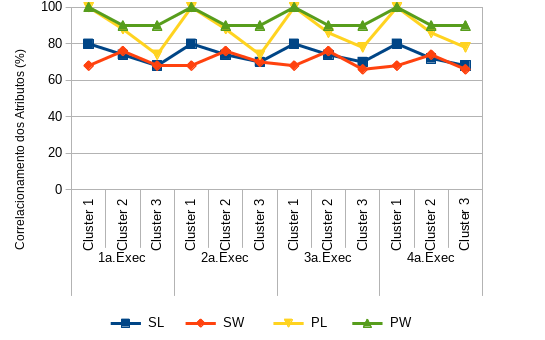
\includegraphics[scale=0.9]{figs/grafico_CART_IRIS_exec_grp.png}
  %      \label{fig:graf:IRIS_CART} }
  %  
  %  \caption{Gráfico de Execuções dos algoritmos supervisionados na base de dados IRIS.} \label{fig:graf:IRIS_NB_CART}
        
  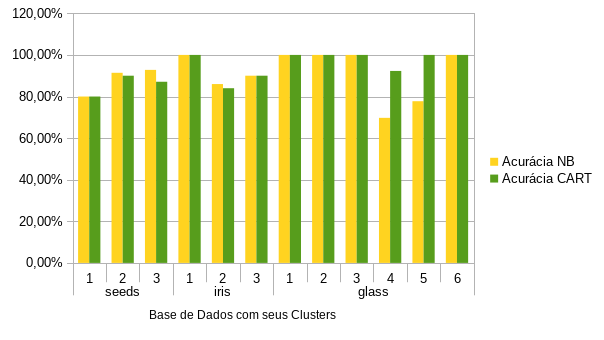
\includegraphics[scale=1]{figs/grafico_NB_CART_acuracia.png}
  \caption{Acurácia por Clusters (Os clusters estão numerados em ordem crescente em cada Base de Dados)} \label{fig:graf:grafico_NB_CART_acuracia}
\end{figure}

No trabalho de \citeonline{LOPES2014} é utilizado um processo de agrupamento da dados para criação de clusters, portanto seus clusters diferem em números de registros comparado ao desta pesquisa. 

%Em relação aos resultados desta pesquisa  pode-se comparar ao trabalho de \citeonline{LOPES2014}, mas em algumas situações não é possível compará-los, por questões de diferenças dos clusters. Existem clusters que não possuem os mesmos números de registros, impossibilitando uma comparação justa. No trabalho do autor citado, é utilizado também um algoritmo de agrupamento de dados, diferente desta pesquisa, que já utiliza os clusters agrupados sem a necessidade de utilizar tal algoritmo. %Essa diferença entre os trabalhos faz com que em determinadas situações não seja possível comparar os resultados.

Por apresentar essas características, resolveu-se apresentar uma tabela comparativa onde o principal argumento é o número de registros que não estão sendo representados pelo rótulo denominado nas colunas das tabelas como \textbf{Fora da Faixa} ou \textbf{Erro}, em razão disso  será possível fazer comparações entre os trabalhos.

% 

A métrica destacada nesta análise comparativa, na base de dados SEEDS, leva em consideração o total de erros. Nesta situação as tabelas \ref{tab:resultado:seeds:nb} e \ref{tab:resultado:seeds:cart} obtiveram um número menor de erros, atestando que o modelo desta pesquisa adquiriu bons resultados em comparação a tabela \ref{tab:resultado:seeds:rn}.


\begin{table}[]
\centering
\caption{Resultado da rotulação utilizando Redes Neurais \cite{LOPES2014}  referente a base de dados SEEDS.}
\label{tab:resultado:seeds:rn}
\begin{tabular}{|c|c|c|c|}
\hline
\rowcolor[HTML]{EFEFEF} 
Cluster             & Num\_Elem             & Atributo & Erro \\ \hline
                    &                      & A        & 8    \\ \cline{3-4} 
\multirow{-2}{*}{1} & \multirow{-2}{*}{67} & P        & 9    \\ \hline
                    &                      & A        & 12   \\ \cline{3-4} 
\multirow{-2}{*}{2} & \multirow{-2}{*}{82} & P        & 10   \\ \hline
                    &                      & P        & 0    \\ \cline{3-4} 
                    &                      & WK       & 3    \\ \cline{3-4} 
                    &                      & LK       & 1    \\ \cline{3-4} 
\multirow{-4}{*}{3} & \multirow{-4}{*}{61} & A        & 0    \\ \hline
\multicolumn{3}{|c|}{Total}                           & 43   \\ \hline
\end{tabular}
\end{table}

\begin{table}[]
\centering
\caption{Resultado da rotulação utilizando Naive Bayes  referente a base de dados SEEDS.}
\label{tab:resultado:seeds:nb}
\begin{tabular}{|c|c|c|c|}
\hline
\rowcolor[HTML]{EFEFEF} 
Cluster             & Num\_Elem             & Atributo & Erro \\ \hline
1                   &    70                & A        & 14    \\ \hline
2                   &   70                 & A        & 6   \\ \hline 
3 &                     70                 & P        & 5   \\ \hline
\multicolumn{3}{|c|}{Total}                           & 25   \\ \hline
\end{tabular}
\end{table}

\begin{table}[]
\centering
\caption{Resultado da rotulação utilizando CART  referente a base de dados SEEDS.}
\label{tab:resultado:seeds:cart}
\begin{tabular}{|c|c|c|c|}
\hline
\rowcolor[HTML]{EFEFEF} 
Cluster             & Num\_Elem             & Atributo & Erro \\ \hline
1                   &    70                & P        & 14    \\ \hline
                    &                    & A        & 6   \\  \cline{3-4}
\multirow{-2}{*}{2} &   \multirow{-2}{*}{70}                 & P        & 7   \\ \hline 
3 &                     70                 & WK        & 9   \\ \hline
\multicolumn{3}{|c|}{Total}                           & 36   \\ \hline
\end{tabular}
\end{table}

%\section*{Trabalhos Futuros}
%\addcontentsline{toc}{chapter}{Trabalhos Futuros}
\section{Trabalhos Futuros}\label{cap:fut}

A pesquisa ainda precisa de mais divulgação na esfera acadêmica, e para isso a publicação de um artigo sobre os resultados apresentados aqui é uma consolidação dessa proposta de mestrado já voltada para a dissertação propriamente dita.

Fazer testes com mais bases de dados  provando que esse método pode ser utilizado em várias bases com características  diferentes.
%Fazer testes com mais bases de dados  e com isso traçar uma estratégia caso seja necessário a utilização da idéia de rotulação por algum fim. Caso algum órgão/setor/empresa precise utilizar a rotulação em seu meio, seria interessante o analista de dados,  saber com quais algoritmos supervisionados ele obteria melhores resultados. Embora se saiba nesse estudo que quaisquer algoritmos supervisionados são capazes de realizar a rotulação de dados, também foi provado que em algumas bases um algoritmo se sobressai a outro. Por consequencia disso ter um maior número de base com características diferentes ajudaria em uma tomada de decisão.

Outro ponto importante é inserir nos teste mais algoritmos, que pertençam a  paradigmas diferentes dos que já foram utilizados.

%* de acordo com autor PEARSON, onde os paradigmas são divididos em :  ...... pode-se perceber que existe uma proximidade na afirmação de rotulação para quaisquer algoritmo supervisionado, não sendo ainda possível afirmar esse tema, por falta de testes em alguns algoritmos de paradigmas ainda não testados, mas já deixando par atrabalhos futuros



%\section*{Cronograma}
%\addcontentsline{toc}{chapter}{Cronograma}
\section{Cronograma}\label{cap:cron}

\definecolor{midgray}{gray}{.8}
\begin{table}[!htbp]
\caption{Cronograma de atividades}     % mude aqui para seu título da tabela
\begin{center}

% %  \resizebox{\textwidth}{!}{ % abre resizebox, setar tabela da largura da página.

\scalebox{1}{
\begin{tabular}{p{6cm}lll}
\hline
\multicolumn{1}{c}{\multirow{2}{*}{Atividades}} & \multicolumn{3}{c}{Meses} \\ \cline{2-4}
\multicolumn{1}{c}{} & Junho & Julho & Agosto    \\ \hline \hline
%\rowcolor[HTML]{EFEFEF}
\footnotesize 1. Testes com Novas Bases de Dados  & \cellcolor{midgray} ~~~~~~~~~ & \cellcolor{midgray} ~~~~~~~~~ & \cellcolor{midgray}~~~~~~~~~  \\ \hline
\footnotesize 2. Modificar Números de Faixa (R) & \cellcolor{midgray} ~~~~~~~~~ & \cellcolor{midgray}~~~~~~~~ & \cellcolor{midgray}~~~~~~~~~  \\ \hline
\footnotesize 3. Testar com outros Algoritmos & \cellcolor{midgray}~~~~~~~~~ & \cellcolor{midgray} ~~~~~~~~~ & \cellcolor{midgray} ~~~~~~~~~ \\ \hline
\footnotesize 4. Preparar Artigo   & ~~~~~~~~~  &  ~~~~~~~~~ & \cellcolor{midgray}  ~~~~~~~~~ \\ \hline
\footnotesize 5. Escrita da Dissertação & ~~~~~~~~~  & ~~~~~~~~~ & \cellcolor{midgray}~~~~~~~~~  \\ \hline
\hline
\end{tabular}
} % fecha resizebox
\end{center}
\label{cronograma} % para referencia no texto.
\end{table}


No primeiro ítem, serão adicionados testes com novas bases que possuam características diferentes quanto ao balanceamento de atributos, bases com muito atributos, bases com muito registros verificando a viabilidade de processamento. 

No segundo ítem serão realizados mais teste com números de faixas diferentes, pois com o processo de discretização o número de faixa poderá influenciar diretamente no ganho de informação.

No terceiro ítem seria a realização de testes com novos algoritmos suportados pela \textit{Statistic and Machine Learning Toolbox} e comparar os resultados.

No último mês seria a dedicação para preparação da dissertação deste trabalho(ítem quatro), e por fim, a escrita de um artigo referente a rotulação de dados (ítem 5) com os testes apresentados nesta pesquisa.

